\documentclass[a4paper,12pt]{article}
%%%%%%%%%%%%%%%%%%%%%%%%%%%%%%%%%%%%%%%%%%%%%%%%%%%%%%%%%%%%%%%%%%%%%%%%%%%%%%%%%%%%%%%%%%%%%%%%%%%%%%%%%%%%%%%%%%%%%%%%%%%%%%%%%%%%%%%%%%%%%%%%%%%%%%%%%%%%%%%%%%%%%%%%%%%%%%%%%%%%%%%%%%%%%%%%%%%%%%%%%%%%%%%%%%%%%%%%%%%%%%%%%%%%%%%%%%%%%%%%%%%%%%%%%%%%
\usepackage{eurosym}
\usepackage{vmargin}
\usepackage{amsmath}
\usepackage{graphics}
\usepackage{epsfig}
\usepackage{framed}
\usepackage{subfigure}
\usepackage{fancyhdr}

\setcounter{MaxMatrixCols}{10}
%TCIDATA{OutputFilter=LATEX.DLL}
%TCIDATA{Version=5.00.0.2570}
%TCIDATA{<META NAME="SaveForMode"CONTENT="1">}
%TCIDATA{LastRevised=Wednesday, February 23, 201113:24:34}
%TCIDATA{<META NAME="GraphicsSave" CONTENT="32">}
%TCIDATA{Language=American English}

\pagestyle{fancy}
\setmarginsrb{20mm}{0mm}{20mm}{25mm}{12mm}{11mm}{0mm}{11mm}
\lhead{Advanced Data Modelling} \rhead{Logistic Regression} \chead{MA4128} %\input{tcilatex}

%http://www.electronics.dit.ie/staff/ysemenova/Opto2/CO_IntroLab.pdf
\begin{document}

\tableofcontents
\newpage
\section{Logistic Regression}
Logistic regression determines the impact of multiple independent variables
presented simultaneously to predict membership of one or other of the two
dependent variable categories.

\subsection{The purpose of logistic regression}
The crucial limitation of linear regression is that it cannot deal with Dependent Variables�s that are \textbf{\textit{dichotomous}} and categorical. Many interesting variables in the business world are dichotomous: for
example, consumers make a decision to buy or not buy (\textit{\textbf{Buy/Don't Buy}}), a product may pass or fail quality control (\textit{\textbf{Pass/Fail}}), there are good or poor credit risks (\textit{\textbf{Good/Poor}}), an employee may be promoted or not (\textit{\textbf{Promote/Don't Promote}}).


A range of regression techniques have been developed for analysing data with categorical dependent
variables, including logistic regression and discriminant analysis (Hence referred to as DA, which is the next section of course).

Logistical regression is regularly used rather than discriminant analysis when there are only two categories
for the dependent variable. Logistic regression is also easier to use with SPSS than DA when
there is a mixture of numerical and categorical Independent Variables�s, because it includes procedures for
generating the necessary dummy variables automatically, requires fewer assumptions, and
is more statistically robust. DA strictly requires the continuous independent variables  (though dummy variables can be used as in multiple regression). Thus, in instances where
the independent variables are categorical, or a mix of continuous and categorical, and the
DV is categorical, logistic regression is necessary.

\subsection{Use of Binomial Probability Theory}
Since the dependent variable is dichotomous we cannot predict a numerical value for it
using logistic regression, so the usual regression least squares deviations criteria for best fit
approach of minimizing error around the line of best fit is inappropriate.

Instead, logistic regression employs binomial probability theory in which there are only two values to
predict: that probability (p) is 1 rather than 0, i.e. the event/person belongs to one group
rather than the other. Logistic regression forms a best fitting equation or function using the
maximum likelihood method (not part of course), which maximizes the probability of classifying the observed
data into the appropriate category given the regression coefficients.
	
	\section{Introduction to Logistic Regression}
	\begin{itemize}
		\item Logistic regression or logit regression is a type of probabilistic statistical classification model.
		
		\item It is also used to predict a binary response from a binary predictor, used for predicting the outcome of a categorical dependent variable (i.e., a class label) based on one or more predictor variables (features). 
		
		\item That is, it is used in estimating empirical values of the parameters in a qualitative response model. The probabilities describing the possible outcomes of a single trial are modeled, as a function of the explanatory (predictor) variables, using a logistic function. 
		
		\item Logistic regression, also called a logit model, is used to model \textbf{dichotomous (i.e. Binary) outcome variables}. In the logit model the log odds of the outcome is modeled as a linear combination of the predictor variables.
		
		\item 
		Binary Logistic regression is used to determine the impact of multiple independent variables
		presented simultaneously to predict membership of one or other of the two
		dependent variable categories.
		\item Logistic regression determines the impact of multiple independent variables
		presented simultaneously to predict membership of one or other of the two
		dependent variable categories.
		\item However, if your dependent variable was not measured on a dichotomous scale, but a continuous scale instead, you will need to carry out \textbf{multiple regression}, whereas if your dependent variable was measured on an ordinal scale, \textbf{ordinal regression} would be a more appropriate starting point.
	\end{itemize}
	
	
	
	\section*{Introduction to Logistic Regression}
	
	The term �\textbf{\textit{generalized linear model}}� is used to describe a procedure for
	transforming the dependent variable so that the �right hand side� of the model
	equation can be interpreted as a \textbf{�\textit{linear combination}}� of the explanatory variables. 	In logistic regression, the logit may be computed in a manner similar to linear regression:
	\[ \eta_i = \beta_0 + \beta_1x_1 + \beta_2x_2 + \ldots  \]
	
	In situations where the dependent (y) variable is continuous and can be
	reasonably assumed to have a normal distribution we do not transform the y
	variable at all and we can simply run a multiple linear regression analysis.
	
	Otherwise some sort of transformation is applied.
	
	
	%---------------------------------------------------------------%
	\subsection{Binomial Logistic Regression} 
	A binomial logistic regression (often referred to simply as logistic regression), predicts the probability that an observation falls into one of two categories of a \textbf{dichotomous} dependent variable based on one or more independent variables that can be either continuous or categorical.
	
	% \section{Binomial Logistic Regression}
	Binomial logistic regression estimates the probability of an event (as an example, having heart disease) occurring. 
	\begin{itemize}
		\item If the estimated probability of the event occurring is greater than or equal to 0.5 (better than even chance), the procedure classifies the event as occurring (e.g., heart disease being present). \item If the probability is less than 0.5, Logistic regression classifies the event as not occurring (e.g., no heart disease). 
	\end{itemize}
	
	\subsection{Examples of Logistic Regression}
	
	\begin{description}
		\item[Example 1:]  Suppose that we are interested in the factors that influence whether a political candidate wins an election.  The outcome (response) variable is binary (0/1); \textit{ win or lose}.  The predictor variables of interest are the amount of money spent on the campaign, the amount of time spent campaigning negatively and whether or not the candidate is an incumbent.
		
		\item[Example 2:]  A researcher is interested in how variables, such as GRE (Graduate Record Exam scores), GPA (grade point average) and prestige of the undergraduate institution, effect admission into graduate school. The response variable, \textit{admit/don't admit}, is a binary variable.
	\end{description}
	
	%You could use binomial logistic regression to understand whether exam performance can be predicted based on revision time, test anxiety and lecture attendance (i.e., where the dependent variable is ``exam performance", measured on a dichotomous scale ? ``passed" or ``failed" ? and you have three independent variables: ``revision time", ``test anxiety" and ``lecture attendance"). 
	%
	%
	%Alternately, you could use binomial logistic regression to understand whether drug use can be predicted based on prior criminal convictions, drug use amongst friends, income, age and gender (i.e., where the dependent variable is ``drug use", measured on a dichotomous scale ? ``yes" or ``no" ? and you have five independent variables: ``prior criminal convictions", ``drug use amongst friends", ``income", ``age" and "gender").
	\newpage
	\subsection{Assumptions}
	
	\begin{description}
		\item[Assumption 1:] Your dependent variable should be measured on a \textbf{dichotomous scale}. Examples of dichotomous variables include gender (two groups: "males" and "females"), presence of heart disease (two groups: "yes" and "no"), personality type (two groups: "introversion" or "extroversion"), body composition (two groups: "obese" or "not obese"), and so forth. \\
		\newline
		
		
		\item[Assumption 2:] You have one or more independent variables, which can be either continuous (i.e., an interval or ratio variable) or categorical (i.e., an ordinal or nominal variable). 
		
		
		
		\item[Assumption 3:] You should have independence of observations and the dependent variable should have mutually exclusive and exhaustive categories.
		
		\item[Assumption 4:] There needs to be a linear relationship between any continuous independent variables and the logit transformation of the dependent variable. 
	\end{description}
	
	%----------------------------------------------------------------------------------------%
	
	\begin{framed}
		\subsection*{Types of Variables (Revision)}
		\begin{itemize}
			\item Examples of \textbf{continuous variables} include revision time (measured in hours), intelligence (measured using IQ score), exam performance (measured from 0 to 100), weight (measured in kg), and so forth. 
			
			\item Examples of \textbf{ordinal variables} include \textit{Likert} items (e.g., a 7-point scale from "strongly agree" through to "strongly disagree"), amongst other ways of ranking categories (e.g., a 3-point scale explaining how much a customer liked a product, ranging from "Not very much" to "Yes, a lot"). 
			\item Examples of \textbf{nominal variables} include gender (e.g., 2 groups: male and female), ethnicity (e.g., 3 groups: Caucasian, African American and Hispanic), profession (e.g., 5 groups: surgeon, doctor, nurse, dentist, therapist), and so forth.
		\end{itemize}
	\end{framed}
	
	
	
	
	
	
	\section{Logistic Regression}
	Logistic regression, also called a logit model, is used to model \textbf{dichotomous outcome} variables. 
	In the logit model the \textbf{log odds} of the outcome is modeled as a linear combination of the predictor variables.
	
	In logistic regression theory, the predicted dependent variable is a function of the probability that a particular subject will be in one of the categories (for example, the probability that a patient has the disease, given his or her set of scores on the predictor variables).
	%------------------------------------------------------------------------------------------------------------------------- %
	\subsection{Logistic Regression: Odds Ratio}
	What are odds?
	The odds of outcome 1 versus outcome 2 are the probability (or frequency) of outcome 1 divided by the probability (or frequency) of outcome 2.
	
	
	\[ \hat{Y} = \frac{\mbox{Odds}}{1+\mbox{Odds}} \]
	
	
	Loglinear models essentially define a pattern of odds ratios, apply the marginals to them, and compare the resulting table with the observed table, in pretty much the same way we apply the Pearson  $\chi^2$ test for association. The big difference is the pattern we define can be much more complicated than independence.
	%---------------------------------------------------------- %
	\subsection{Odds}
	The odds in favor of an event or a proposition are the ratio of the probability that an event will happen to the probability that it will not happen.
	'Odds' are an expression of relative probabilities. Often 'odds' are quoted as odds against, rather than as odds in favor of, because of the possibility of confusion of the latter with the fractional probability of an event occurring.
	\[ \operatorname{Odds} = \frac{p}{1-p} \]
	
	\subsubsection{Example}
	There are 5 pink marbles, 2 blue marbles, and 8 purple marbles.
	
	\begin{itemize}
		\item What is the probability of picking a blue marble? (Answer: 2/15).
		\item What are the odds in favor of picking a blue marble? (Answer: 2/13).
	\end{itemize}
	
	
	
	%--------------------------------------------%
	
	\subsection{Introduction to the Odds Ratio}
	Let's begin with probability. Suppose that the probability of success is 0.8, thus
	p = 0.8
	Then the probability of failure is
	\[q = 1 - p = 0.2\]
	The odds of success are defined as
	\[odds(success) = p/q = 0.8/0.2 = 4\]
	that is, the odds of success are 4 to 1. The odds of failure would be
	\[odds(failure) = q/p = .2/.8 = .25\]
	This looks a little strange but it is really saying that the odds of failure are 1 to 4.  The odds of success and the odds of failure are just reciprocals of one another, i.e., 1/4 = .25 and 1/.25 = 4. 
	
	
	Next, we will add another variable to the equation so that we can compute an odds ratio.
	
	\noindent  \textbf{Another example}
	
	Suppose that seven out of 10 males are admitted to an engineering school while three of 10 females are admitted. 
	
	\begin{itemize}
		\item The probabilities for admitting a male are,
		p = 7/10 = 0.7      ( q = 1 - 0.7 = 0.3)
		\item Here are the same probabilities for females,
		p = 3/10 = 0.3       (q = 1 - 0.3 = 0.7)
	\end{itemize}
	Now we can use the probabilities to compute the admission odds for both males and females,
	\begin{itemize}
		\item \textit{odds(male) }= 0.7/0.3 = 2.33333
		\item \textit{odds(female) }= 0.3/0.7 = 0.42857
	\end{itemize}
	Next, we compute the odds ratio for admission,
	\[OR = 2.3333/0.42857 = 5.44\]
	Thus, for a male, the odds of being admitted are 5.44 times as large than the odds for a female being admitted.
	
	\subsection{Odds Ratio Example}
	These data are taken from the British Election Study 2005 pre-campaign and
	post-election panel data. We will consider the propensity to vote (sometimes called �turnout�) as the
	dependent variable, which has 2 categories. 0=did not turn out to vote, 1 turned
	out to vote.
	
	\begin{center}
		\begin{figure}[h!]
			% Requires \usepackage{graphicx}
			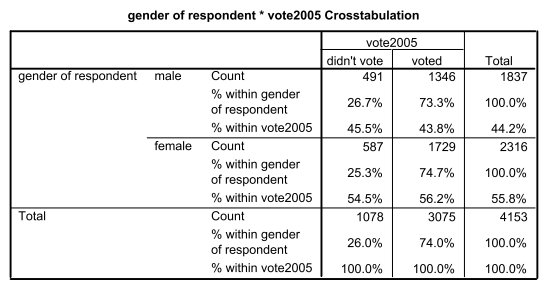
\includegraphics[scale=0.8]{LogWeek10A}\\
			\caption{General Election 2005}
		\end{figure}
	\end{center}
	
	% Image LogWeek10-A
	
	The odds of a male turning out to vote are:
	\[1346/491 = 2.741\]
	The odds of female turning out to vote are
	\[1729/587 = 2.945\]
	The Odds ratio (female: male) are
	(1729/587) / (1346/491) = 1.074
	
	\subsection{Logistic Regression: Odds Ratios and Log-Odds}
	\begin{itemize}
		\item Suppose that in a sample of 100 men, 90 drank wine in the previous week, while in a sample of 100 women only 20 drank wine in the same period. \item The odds of a man drinking wine are 90 to 10, or 9:1, while the odds of a woman drinking wine are only 20 to 80, or 1:4 = 0.25:1. 
		\item The odds ratio is thus 9/0.25, or 36, showing that men are much more likely to drink wine than women. 
		\item The detailed calculation is:
		
		
		\[ { 0.9/0.1 \over 0.2/0.8}=\frac{\;0.9\times 0.8\;}{\;0.1\times 0.2\;} ={0.72 \over 0.02} = 36 \]
		
		\item This example also shows how odds ratios are sometimes sensitive in stating relative positions: in this sample men are 90/20 = 4.5 times more likely to have drunk wine than women, but have 36 times the odds. 
		
		
		
		\item The logarithm of the odds ratio, the difference of the logits of the probabilities, tempers this effect, and also makes the measure symmetric with respect to the ordering of groups. 
		\item For example, using natural logarithms, an odds ratio of 36/1 maps to 3.584, and an odds ratio of 1/36 maps to -3.584.
	\end{itemize}
	
	
	
	
	
	
	
	
	%-------------------------------------------%
	
	
	\subsubsection{Confidence Intervals for Odds Ratios}
	\begin{itemize}
		\item Many statistical implementations of logistic regression include Confidence Intervals for the odds ratios.
		Odds ratios whose confidence limits exclude 1 are statistically significant.
		\item The odds ratio is referred to in SPSS as \texttt{\textbf{Exp(B)}}, the exponentiation of the B coefficient
	\end{itemize}
	
	%-------------------------------------------%
	\subsection{Log-Odds}
	As an alternative to modeling the value of the outcome, logistic regression focuses instead upon the
	relative probability (odds) of obtaining a given result category. The natural logarithm of the odds is
	linear across most of its range, allowing us to continue using many of the methods developed for linear models.
	The result of this type of regression can be expressed as follows:
	\[ \operatorname{Ln} \left[ \frac{p}{1-p} \right] = b_0 + b_1x_1 + b_2x_2 + b_3x_3 \ldots b_kx_k + e \]
	
	%-------------------------------------------%
	
	\subsection{About logits}
	
	
	There is a direct relationship between the coefficients produced by \textbf{logit} and the odds ratios produced by the logistic procedure.  First, let's define what is meant by a logit:  A logit is defined as the log base e (log) of the odds,
	\[logit(p) = log(odds) = log(p/q)\]
	Logistic regression is in reality ordinary regression using the logit as the response variable,
	
	\[logit(p) = log(p/q) = b_0 + b_1X\]
	
	This means that the coefficients in logistic regression are in terms of the log odds, that is, the coefficient 1.694596 implies that a one unit change in gender results in a 1.694596 unit change in the log of the odds.  
	
	Equation [3] can be expressed in odds by getting rid of the log.  This is done by taking e to the power for both sides of the equation.
	\[ p/q = e^{b_0 + b_1}\]
	The end result of all the mathematical manipulations is that the odds ratio can be computed by raising e to the power of the logistic coefficient,
	\[OR = e^b = e^1.694596 = 5.44\]
	
	
	%---------------------------------------------------------- %
	\newpage
	
	\subsection{The Sigmoid Graph}
	While logistic regression gives each predictor (IV) a coefficient \textbf{b} which measures its
	independent contribution to variations in the dependent variable, the dependent variable
	can only take on one of the two values: 0 or 1.
	
	What we want to predict from a knowledge of relevant independent variables and coefficients is therefore not a numerical value of a
	dependent variable as in linear regression, but rather the probability (p) that it is 1 rather
	than 0 (belonging to one group rather than the other). But even to use probability as the dependent variable is unsound, mainly because numerical predictors may be unlimited in range. If we expressed p as a linear function of investment, we might then find ourselves predicting that p is greater than 1 (which cannot be true, as
	probabilities can only take values between 0 and 1). Additionally, because logistic regression
	has only two y values � in the category or not in the category � a straight line best fit (as in
	linear regression) is not possible to draw.
	\subsubsection{Hypothetical Example}
	Consider the following hypothetical example:
	200 accountancy first year students are graded on a pass-fail dichotomy on the end of the
	semester accountancy exam. At the start of the course, they all took a maths pre-test with
	results reported in interval data ranging from 0�50 � the higher the pretest score the more
	competency in maths. Logistic regression is applied to determine the relationship between
	maths pretest score (IV or predictor) and whether a student passed the course (DV). Students
	who passed the accountancy course are coded 1 while those who failed are coded 0.
	\begin{center}
		\begin{figure}[h!]
			% Requires \usepackage{graphicx}
			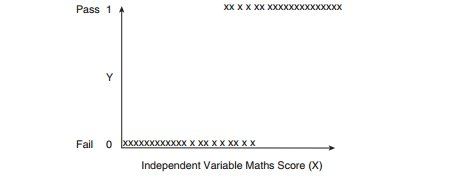
\includegraphics[scale=1.1]{images/Logistic1}\\
			\caption{Accountancy Exam Results}
		\end{figure}
	\end{center}
	
	We can see from Figure 1 of the plotted �x�s� that there is somewhat greater likelihood
	that those who obtained above average to high score on the maths test passed the accountancy course, while below average to low scorers tended to fail. There is also an overlap in
	the middle area. But if we tried to draw a straight (best fitting) line, as with linear regression,
	it just would not work, as intersections of the maths results and pass/fail accountancy results
	form two lines of x�s, as in Figure 1.
	%
	%\begin{figure}
	%  % Requires \usepackage{graphicx}
	%  \includegraphics[width=0.40]{Logistic2.jpeg}\\
	%  \caption{Figure 2}
	%\end{figure}
	\begin{center}
		\begin{figure}
			% Requires \usepackage{graphicx}
			\includegraphics[scale=0.8]{images/Logistic2}\\
			\caption{Accountancy Exam Results - Fitted Curve}
		\end{figure}
	\end{center}
	
	The solution is to convert or transform these results into probabilities. We might compute
	the average of the Y values at each point on the X axis. We could then plot the probabilities
	of Y at each value of X and it would look something like the wavy graph line superimposed
	on the original data in Figure 2. This is a smoother curve, and it is easy to see that the
	probability of passing the accountancy course (Y axis) increases as values of X increase.
	What we have just done is transform the scores so that the curve now fits a cumulative
	probability curve, i.e. adding each new probability to the existing total. As you can see, this
	curve is not a straight line; it is more of an s-shaped curve (A sigmoid curve).
	
	Predicted values are interpreted as probabilities and are now not just two conditions with a value of either 0 or 1 but continuous data that can take any value from 0 to 1.
	The slope of the curve in Figure 2 is low at the lower and upper extremes of the
	independent variable and greatest in the middle where it is most sensitive. In the middle, of
	course, are a number of cases that are out of order, in the sense that there is an overlap with
	average maths scores in both accountancy pass and fail categories, while at the extremes are
	cases which are almost universally allocated to their correct group. The outcome is not a prediction of a Y value, as in linear regression, but a probability of belonging to one of two conditions
	of Y, which can take on any value between 0 and 1 rather than just 0 and 1 in Figure 1.
	
	\subsubsection{Log transformation}
	Unfortunately a further mathematical transformation � a log transformation � is needed
	to normalize the distribution. Transformations, such as log transformations and
	square root transformations transform non-normal/skewed distributions closer to normality.
	
	This log transformation of the p values to a log distribution enables us to create a link with the normal regression equation. The log distribution (or logistic transformation of p) is also called the logit of p or \textbf{\textit{logit(p)}}.
	
	\newpage
	\subsection{The Logit}
	The convention for binomial logistic regression is to code the
	dependent class of greatest interest as 1 and the other class as 0, because the coding will
	affect the odds ratios and slope estimates.
	
	The logit(p) is the log (to base e) of the odds ratio or likelihood ratio that the dependent
	variable is 1. In symbols it is defined as:
	\[ logit(p) = ln \left(\frac{p}{(1-p)}\right) \]
	
	Whereas p can only range from 0 to 1, logit(p) scale ranges from negative infinity to positive
	infinity and is symmetrical around the logit of 0.5 (which is zero)
	
	\subsection{The Logistic Regression Equation}
	The form of the logistic regression equation is:
	\begin{framed}
		\[ \mbox{logit}[p(x)] =  log \left(\frac{p(x)}{1-p(x)} \right) = b_0 + b_1x_1 + b_2x_2 + b_3x_3 + \ldots \]
	\end{framed}
	This looks just like a linear regression and although logistic regression finds a �best
	fitting� equation, just as linear regression does, the principles on which it does so are
	rather different. Instead of using a least-squared deviations criterion for the best fit, it
	uses a maximum likelihood method, which maximizes the probability of getting the
	observed results given the fitted regression coefficients. A consequence of this is that the
	goodness of fit and overall significance statistics used in logistic regression are different
	from those used in linear regression.
	
	The probability that a case is in a particular category,p, can be calculated with the following formula (which is simply another rearrangement of the previous formula).
	
	\[p = \frac{exp(b_0 + b_1x_1 + b_2x_2 + b_3x_3 + \ldots)}{1 + exp(b_0 + b_1x_1 + b_2x_2 + b_3x_3 + \ldots)}\]
	
	\newpage
	
	\section*{Logistic function} 
	
	The logistic function, with $\beta_0 + \beta_1 x$ on the horizontal axis and $\pi(x)$ on the vertical axis
	An explanation of logistic regression begins with an explanation of the logistic function, which always takes on values between zero and one:
	\[
	F(t) = \frac{e^t}{e^t+1} = \frac{1}{1+e^{-t}},
	\]
	and viewing t as a linear function of an explanatory variable x (or of a linear combination of explanatory variables), the logistic function can be written as:
	\[\pi(x) = \frac{e^{(\beta_0 + \beta_1 x)}} {e^{(\beta_0 + \beta_1 x)} + 1} = \frac {1} {1+e^{-(\beta_0 + \beta_1 x)}}.
	\]
	This will be interpreted as the probability of the dependent variable equalling a ``success" or ``case" rather than a failure or non-case. We also define the inverse of the logistic function, the logit:
	\[g(x) = \ln \frac {\pi(x)} {1 - \pi(x)} = \beta_0 + \beta_1 x ,
	\]and equivalently:
	\[\frac{\pi(x)} {1 - \pi(x)} = e^{(\beta_0 + \beta_1 x)}.
	\]
	%======================================================%
	
	\section{Logistic Regression: Logits}
	%http://data.princeton.edu/wws509/notes/c3.pdf
	
	The logit transformation is given by the following formula: 
	\[ \eta_i = \mbox{logit}(p_i)  = \mbox{log}\left( \frac{p_i}{1- p_i} \right) \]
	
	To inverse of the logit transformation is given by the following formula: 
	\[ p_i = \mbox{logit}^{-1}(\eta_i)  =  \frac{e^{\eta_i}}{1 + e^{\eta_i}} \]
	
	%---------------------------%
	
	
	\section{Review of Logistic Regression}
	% http://www.nesug.org/proceedings/nesug06/an/da26.pdf
	% http://www.ccsr.ac.uk/publications/teaching/blr.pdf
	% http://www.southampton.ac.uk/ghp3/docs/unicef/presentation7.1a.pdf
	% ftp://public.dhe.ibm.com/software/analytics/spss/documentation/statistics/20.0/en/client/Manuals/IBM_SPSS_Regression.pdf
	% http://www.umass.edu/statdata/statdata/data/
	
	%---------------------------------------------------------------%
	
	
	\subsection*{Example 1}
	Given that $\pi_i = 0.2$, compute $\eta_i$.
	
	\[ \eta_i = \mbox{log}\left( \frac{0.2}{1-0.2} \right)= \mbox{log}\left( \frac{0.2}{0.8} \right)\] 
	
	\[ \eta_i =  \mbox{log}(0.25) =-1.386 \]
	
	%---------------------------%
	\subsection{Example 2}
	Let us suppose that the probability of survival of a marine species of fauna is dependent on pollution, depth and water temperature. Suppose the logit for the logistic regression was computed as follows:
	\[ \eta_i = 0.14 + 0.76x_1 - 0.093x_2 + 1.2x_3  \]
	\begin{center}
		\begin{tabular}{|c|c|c|}
			\hline
			% after \\: \hline or \cline{col1-col2} \cline{col3-col4} ...
			Variables & case 1 & case 2 \\ \hline
			Pollution($x_1$) & 6.0 & 1.9 \\
			Depth ($x_2$)& 51 & 99 \\
			Temp ($x_3$) & 3.0 & 2.9 \\
			\hline
		\end{tabular}
	\end{center}
	Compute the probability of success for both case 1 and case 2.
	
	\begin{itemize}
		\item case 1$ \eta_1 = 0.14 + (0.76 \times 6)	- (0.093\times 51) + (1.2\times 3) = 3.557$
		\item case 2$ \eta_2 = 0.14 + (0.76 \times 1.9)	- (0.093\times 99) + (1.2\times 2.9) = -4.143$
	\end{itemize}
	
	The probabilities for success are therefore:
	\[ \pi_1  =  \frac{e^{3.557}}{1 + e^{3.557}} = \frac{35.057}{1 + 35.057} = 0.972 \]
	\[ \pi_2  =  \frac{e^{-4.143}}{1 + e^{-4.143}} = \frac{0.0158}{1 + 0.0158} = 0.0156 \]
	
	
%	
%	\subsection*{Example 2}
%	Given that $\eta_i = 2.3$, compute $\pi_i$.
%	
%	\[ \pi_i  =  \frac{e^{2.3}}{1 + e^{2.3}} = \frac{9.974}{1 + 9.974} = 0.908 \]
	
	%--------------------------------------------------------------------------------------%
	
	\subsection*{Logistic Regression: Logit Transformation}
	%http://data.princeton.edu/wws509/notes/c3.pdf
	
	The logit transformation is given by the following formula: 
	\[ \eta_i = \mbox{logit}(\pi_i)  = \mbox{log}\left( \frac{\pi_i}{1- \pi_i} \right) \]
	
	\noindent 
	The inverse of the logit transformation is given by the following formula: 
	\[ \pi_i = \mbox{logit}^{-1}(\eta_i)  =  \frac{e^{\eta_i}}{1 + e^{\eta_i}} \]
	
	%---------------------------%
	\subsection*{Logits}
	In logistic regression, the logit may be computed in a manner similar to linear regression:
	\[ \eta_i = \beta_0 + \beta_1x_1 + \beta_2x_2 + \ldots  \]
	
	%---------------------------%
	
	
	
	
	\subsection{Logistic function}
	
	The logistic function of any number is given by the inverse-logit:
	
	\[\operatorname{logit}^{-1}(\alpha) = \frac{1}{1 + \operatorname{exp}(-\alpha)} = \frac{\operatorname{exp}(\alpha)}{1 + \operatorname{exp}(\alpha)}\]
	
	%-------------------------------------------%
	
	
	\subsection{Dummy variables}
	When an explanatory variable is categorical we can use \textbf{dummy variables} to contrast
	the different categories. For each variable we choose a baseline category and then
	contrast all remaining categories with the base line. If an explanatory variable
	has k categories, we need k-1 dummy variables to investigate all the differences in
	the categories with respect to the dependent variable.
	
	For example suppose the explanatory variable was \textbf{\textit{housing}} coded like this:
	\begin{itemize}
		\item[1:] Owner occupier
		\item[2:] renting from a private landlord
		\item[3:] renting from the local authority
	\end{itemize}
	
	We would therefore need to choose a baseline category and create two dummy
	variables. For example if we chose owner occupier as the baseline category we
	would code the dummy variables (House1 and House2) like this
	
	%Tenure: &House1 &House2\\
	%Owner occupier &0& 0\\
	%Rented private &1 &0\\
	%Rented local authority &0 &1\\
	
	\subsection{Log Likelihood}
	A ``likelihood" is a probability, specifically the probability that the observed values of the dependent may be predicted from the observed values of the independents. 
	
	Like any probability, the likelihood varies from 0 to 1. The log likelihood (LL) is its log and varies from 0 to minus infinity (it is negative because the log of any number less than 1 is negative). LL is calculated through iteration, using maximum likelihood estimation (MLE).
	
	
	\subsection{Maximum Likelihood Estimation}
	\begin{itemize}
		\item Maximum likelihood estimation, MLE, is the method used to calculate the logit coefficients. This contrasts to the use of ordinary least squares (OLS) estimation of coefficients in regression. OLS seeks to minimize the sum of squared distances of the data points to the regression line. 
		\item MLE seeks to maximize the log likelihood, LL, which reflects how likely it is (the odds) that the observed values of the dependent may be predicted from the observed values of the independents. (Equivalently MLE seeks to minimize the -2LL value.)
		
		\item MLE is an iterative algorithm which starts with an initial arbitrary ``guesstimate" of what the logit coefficients should be, the MLE algorithm determines the direction and size change in the logit coefficients which will increase LL. 
		\item After this initial function is estimated, the residuals are tested and a re-estimate is made with an improved function, and the process is repeated (usually about a half-dozen times) until convergence is reached (that is, until LL does not change significantly). There are several alternative convergence criteria.
	\end{itemize}
	
	
	\subsection{Wald statistic}
	\begin{itemize}
		\item Alternatively, when assessing the contribution of individual predictors in a given model, one may examine the significance of the Wald statistic. The Wald statistic, analogous to the t-test in linear regression, is used to assess the significance of coefficients. 
		
		\item The Wald statistic is commonly used to test the significance of individual logistic regression coefficients for each independent variable (that is, to test the null hypothesis in logistic regression that a particular logit (effect) coefficient is zero). 
		
		\item The Wald Statistic is the ratio of the unstandardized logit coefficient to its standard error. The Wald statistic and its corresponding p probability level is part of SPSS output in the section \textbf{\textit{Variables in the Equation.}} This corresponds to significance testing of b coefficients in OLS regression. The researcher may well want to drop independents from the model when their effect is not significant by the Wald statistic.
		
		
		\item The Wald statistic is the ratio of the square of the regression coefficient to the square of the standard error of the coefficient and is asymptotically distributed as a chi-square distribution.
	\end{itemize}
	% Wald Test?
	
	\subsubsection*{Wald Test}
	The Wald test is a way of testing the signi�cance of particular explanatory variables in a statistical model. In logistic regression we have a binary outcome variable and one or more explanatory variables. For each explanatory variable in the model there will be an associated parameter.
	The Wald test, described by Polit (1996) and Agresti (1990), is one of a number of ways of testing whether the parameters associated with a group of
	explanatory variables are zero.
	
	If for a particular explanatory variable, or group of explanatory variables, the Wald test is significant, then we would conclude that the parameters associated with these variables are not zero, so that the variables should be included in the model. If the Wald test is not significant then these explanatory variables can be omitted from the model. When considering a single explanatory variable, Altman (1991) uses a t-test to check whether the parameter is significant. 
	
	For a single parameter the Wald statistic is just the square of the t-statistic and so will give exactly equivalent results.
	An alternative and widely used approach to testing the significance of a number of explanatory variables is to use the likelihood ratio test. This is
	appropriate for a variety of types of statistical models. Agresti (1990) argues that the likelihood ratio test is better, particularly if the sample size is small or the parameters are large.
	
	\newpage
	
	The Wald Test is a statistical test used to determine whether an effect exists or not,
	
	It tests whether an independent variable has a statistically significant relationship with a dependent variable.
	
	It is used in a great variety of different models including models for dichotomous variables and model for continuous
	variables.
	
	\begin{itemize}
		\item $\hat{\theta}$ Maximum likelihood estimate of the parameter of interest $\theta$
		\item $theta_o$ Proposed value.
		This is an assumption of the fact that the differences between $\hat{\theta}$ and $theta_o$ is normal.
		
		Univariate case
		\[ \frac{(\hat{\theta} - theta_o )^2}{\mbox{var}(\hat{\theta})} \sim \chi^2 \]
		\[ \frac{(\hat{\theta} - theta_o )^2}{\mbox{s.e.}(\hat{\theta})} \sim \mbox{Normal} \]
	\end{itemize}	
	The likelihood ratio test is also used to determine whether an effect exists.
	]
	\newpage
	%-------------------------------------------------------%
	\subsection*{South Africa Heart Disease Data Example}
	
	\begin{framed}
		A retrospective sample of males in a heart-disease high-risk region
		of the Western Cape, South Africa. There are roughly two controls per
		case of CHD. Many of the CHD positive men have undergone blood
		pressure reduction treatment and other programs to reduce their risk
		factors after their CHD event. In some cases the measurements were
		made after these treatments. These data are taken from a larger
		dataset, described in  Rousseauw et al, 1983, South African Medical
		Journal. 
		
	\end{framed}
	%Load the South Africa Heart Disease Data and create training and test sets with
	%the following code:
	%\begin{framed}
	%	\begin{verbatim}
	%	install.packages("ElemStatLearn")
	%	library(ElemStatLearn)
	%	data(SAheart)
	%	
	%	set.seed(8484)
	%	train = sample(1:dim(SAheart)[1],
	%	size=dim(SAheart)[1]/2,replace=F)
	%	trainSA = SAheart[train,]
	%	testSA = SAheart[-train,]
	%	
	%	\end{verbatim}
	%\end{framed}
	
	\noindent \textbf{Exercise}\\Fit a logistic regression model with
	\begin{itemize}
		\item \textit{Coronary Heart Disease} (\texttt{chd}) as the
		dependent variable
		
		\item \textit{age at onset, current alcohol consumption, obesity levels,
			cumulative tabacco, type-A behavior}, and \textit{low density lipoprotein cholesterol} as predictor variables. 
	\end{itemize} 
	{
		\large
		
		\begin{verbatim}
		> head(SAheart)
		sbp tobacco  ldl adiposity famhist typea obesity alcohol age chd
		1 160   12.00 5.73     23.11 Present    49   25.30   97.20  52   1
		2 144    0.01 4.41     28.61  Absent    55   28.87    2.06  63   1
		3 118    0.08 3.48     32.28 Present    52   29.14    3.81  46   0
		4 170    7.50 6.41     38.03 Present    51   31.99   24.26  58   1
		5 134   13.60 3.50     27.78 Present    60   25.99   57.34  49   1
		6 132    6.20 6.47     36.21 Present    62   30.77   14.14  45   0
		...
		...
		\end{verbatim}
		
	}
	\noindent Calculate the misclassification rate for your model using this model
	% function and a prediction on the "response" scale:
	
	%\noindent What is the misclassification rate on the training set? What is the
	%misclassification rate on the test set?
	%\begin{framed}
	%	\begin{verbatim}
	%	head(SAheart)
	%	
	%	lr1 <- glm(chd ~ age + alcohol + obesity + 
	%	tobacco + typea + ldl, data=trainSA, 
	%	family="binomial")
	%	
	%	lr1.train.predict <- predict(lr1, type="response")
	%	
	%	missclass.lr1.train <- missClass(trainSA$chd, 
	%	lr1.train.predict)
	%	
	%	lr1.test.predict <- predict(lr1, newdata=testSA, 
	%	type="response")
	%	
	%	missclass.lr1.test <- missClass(testSA$chd, 
	%	lr1.test.predict)
	%	\end{verbatim}
	%\end{framed}
	
	
	\newpage
	%-------------------------------------------------------%
	
	%------------------------------------------------------------------------------------%
	\section{Wald statistic}
	\begin{itemize}
		\item Alternatively, when assessing the contribution of individual predictors in a given model, one may examine the significance of the Wald statistic. The Wald statistic, analogous to the t-test in linear regression, is used to assess the significance of coefficients. 
		\item The Wald statistic is the ratio of the square of the regression coefficient to the square of the standard error of the coefficient and is asymptotically distributed as a chi-square distribution.[9]
		
		\[W_j = \frac{B^2_j} {SE^2_{B_j}}\]
		
		\item Although several statistical packages (e.g., SPSS, SAS) report the Wald statistic to assess the contribution of individual predictors, the Wald statistic has limitations. 
		\item When the regression coefficient is large, the standard error of the regression coefficient also tends to be large increasing the probability of Type-II error. 
		
		\item The Wald statistic also tends to be biased when data are sparse.
		
	\end{itemize}
	
	%--------------------------------------------------------%
	\begin{figure}[h!]
		\centering
		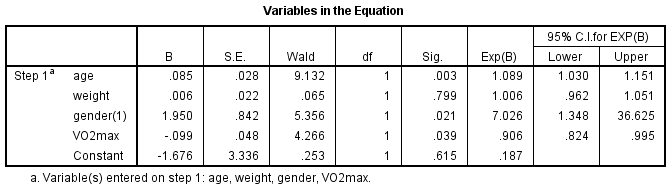
\includegraphics[width=0.7\linewidth]{images/waldtest}
		\caption{}
		\label{fig:waldtest}
	\end{figure}
	
	\subsection{The Wald Test}
	\begin{itemize}
		\item The Wald test is a way of testing the significance of particular predictor variables in a statistical model. 
		
		\item In logistic regression we have a binary outcome variable and one or more explanatory variables. For each predictor variable in the model there will be an associated parameter. The Wald test is one of a number of ways of testing whether the parameters associated with a group of explanatory variables are zero.
		%, described by Polit (1996) and Agresti (1990), 
		
		\item If for a particular explanatory variable, or group of explanatory variables, the Wald test is significant, then we would conclude that the parameters associated with these variables are not zero, so that the variables should be included in the model. If the Wald test is not significant then these explanatory variables can be omitted from the model. 
		
		\item When considering a single explanatory variable, Altman (1991) uses a t-test to check whether the parameter is significant. For a single parameter the Wald statistic is just the square of the t-statistic and so will give exactly equivalent results.
		
		\item An alternative and widely used approach to testing the significance of a number of explanatory variables is to use the likelihood ratio test. This is appropriate for a variety of types of statistical models. 
		
		\item Agresti (1990) argues that the likelihood ratio test is better, particularly if the sample size is small or the parameters are large.
	\end{itemize}
	
	
	
	%-------------------------------------------%
	\newpage
\subsection{Variable Selection}
Like ordinary regression, logistic regression provides a coefficient \textbf{b} estimates, which measures
each IV�s partial contribution to variations in the response variables. The goal is to correctly predict
the category of outcome for individual cases using the most parsimonious model.

To accomplish this goal, a model (i.e. an equation) is created that includes all predictor variables that are useful in predicting the response variable. Variables can, if necessary, be entered into the model in the order specified by the researcher in a stepwise fashion like regression.

There are two main uses of logistic regression:
\begin{itemize}
\item The first is the prediction of group membership. Since logistic regression calculates the
probability of success over the probability of failure, the results of the analysis are in
the form of an \textbf{odds ratio}.
\item Logistic regression also provides knowledge of the relationships and strengths among
the variables (e.g. playing golf with the boss puts you at a higher probability for job
promotion than undertaking five hours unpaid overtime each week).
\end{itemize}

\subsection{Assumptions of logistic regression}
\begin{itemize}
\item Logistic regression does not assume a linear relationship between the dependent and
independent variables.
\item The dependent variable must be a dichotomy (2 categories).
\textit{(Remark: Dichotomous refers to two outcomes. Multichotomous refers to more than two outcomes)}.
\item The independent variables need not be interval, nor normally distributed, nor linearly
related, nor of equal variance within each group.
\item The categories (groups) must be mutually exclusive and exhaustive; a case can only be
in one group and every case must be a member of one of the groups.
\item Larger samples are needed than for linear regression because maximum likelihood
coefficients are large sample estimates. A minimum of 50 cases per predictor is
recommended.
\end{itemize}
%===================================== %
\newpage
\subsection{Odds and Odds Ratio}
Logistic regression calculates changes in the log odds of the dependent,
not changes in the dependent value as OLS regression does. For a dichotomous variable the
odds of membership of the target group are equal to the probability of membership in the
target group divided by the probability of membership in the other group. Odds value can
range from 0 to infinity and tell you how much more likely it is that an observation is a
member of the target group rather than a member of the other group. If the probability is
0.80, the odds are 4 to 1 or 0.80/0.20; if the probability is 0.25, the odds are .33 (0.25/0.75).

If the probability of membership in the target group is 0.50, the odds are 1 to 1 (0.50/0.50), as
in coin tossing when both outcomes are equally likely.

Another important concept is the odds ratio (OR), which estimates the change in the
odds of membership in the target group for a one unit increase in the predictor. It is calculated by using the regression coefficient of the predictor as the exponent. Suppose we were predicting exam success by a maths competency
predictor with an estimate b = 2.69. Thus the odds ratio is exp(2.69) or 14.73. Therefore the odds of passing
are 14.73 times greater for a student, for example, who had a pre-test score of 5, than for a
student whose pre-test score was 4.
%--------------------------------------------------------%

\subsection{Exercise Data Set}
The exercise data set comes from a survey of home owners
conducted by an electricity company about an offer of roof solar panels with a 50\% subsidy
from the state government as part of the state�s environmental policy. The variables involve
household income measured in units of a thousand dollars, age, monthly mortgage, size of
family household, and as the dependent variable, whether the householder would take or decline the offer.
The purpose of the exercise is to conduct a logistic regression to determine whether family
size and monthly mortgage will predict taking or declining the offer.

For the first demonstration, we will use `family size� and
`mortgage� only. For the options, select Classification Plots, Hosmer-Lemeshow Goodness
Of Fit, Casewise Listing Of Residuals and select Outliers Outside 2sd. Retain default
entries for probability of stepwise, classification cutoff and maximum iterations.

\begin{figure}[h!]
\begin{center}
  % Requires \usepackage{graphicx}
  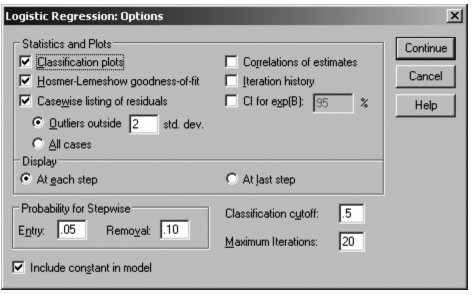
\includegraphics[scale=0.8]{images/Logistic10}\\
  \caption{Selected Options for Exercises}
\end{center}
\end{figure}

We are not using any categorical variables this time. If there are categorical variables, use the \textbf{\textit{categorical}} option. For most situations, choose the �indicator� coding scheme (it is the
default).
\subsection{SPSS Outout  - Block 0: Beginning Block.}
Block 0 presents the results with only the constant included
before any coefficients (i.e. those relating to family size and mortgage) are entered into
the equation. Logistic regression compares this model with a model including all the
predictors (family size and mortgage) to determine whether the latter model is more
appropriate. The table suggests that if we knew nothing about our variables and guessed
that a person would not take the offer we would be correct 53.3\% of the time.
\begin{figure}[h!]
\begin{center}
  % Requires \usepackage{graphicx}
  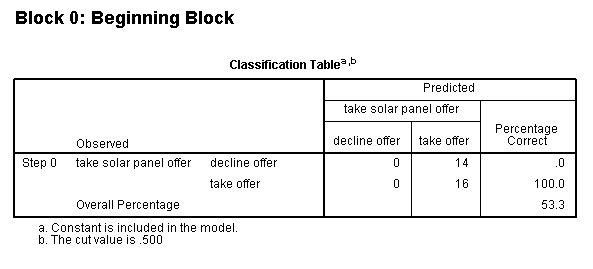
\includegraphics[scale=0.6]{images/Logistic3}\\
  \caption{Classification table}
\end{center}
\end{figure}
The variables not in the equation table tells us whether each IV improves the model. The answer is yes for both variables, with family size slightly better than mortgage size, as both are significant and if included would add to the predictive power of the model. If they had not been significant and able to contribute to the prediction,
then termination of the analysis would obviously occur at this point

\begin{figure}
\begin{center}
  % Requires \usepackage{graphicx}
  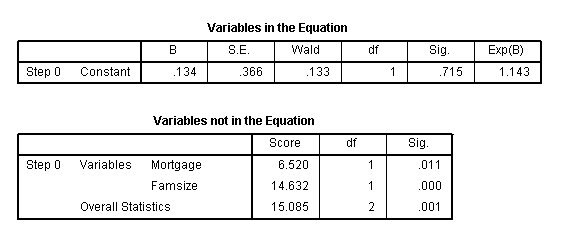
\includegraphics[scale=0.6]{images/Logistic4}\\
  \caption{Variables in / not in the equation}
\end{center}
\end{figure}
This presents the results when the predictors �family size� and
�mortgage� are included. Later SPSS prints a classification table which shows how the
classification error rate has changed from the original 53.3%. By adding the variables
we can now predict with 90\% accuracy (see Classification Table later). The
model appears good, but we need to evaluate model fit and significance as well. SPSS will
offer you a variety of statistical tests for model fit and whether each of the independent
variables included make a significant contribution to the model.
\begin{figure}
\begin{center}
  % Requires \usepackage{graphicx}
  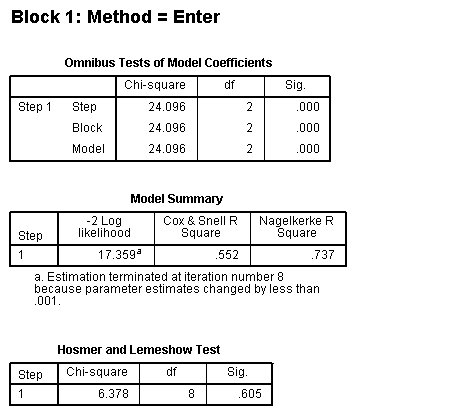
\includegraphics[scale=0.6]{images/Logistic5}\\
  \caption{Test Outcomes}
\end{center}
\end{figure}
\subsection{Omnibus Test for Model Coefficients}
The overall significance is tested using what SPSS calls the \textbf{\textit{Model Chi-square}}, which is derived from the likelihood of observing the actual data under the assumption that the model that has been fitted is accurate. There are two hypotheses to test in relation to the overall fit of the model:


 \begin{itemize}
 \item[$H_0$] The model is a good fitting model.
 \item[$H_1$] The model is not a good fitting model (i.e. the predictors have a significant effect).
 \end{itemize}
 In our case model chi square has 2 degrees of freedom, a value of 24.096 and a probability of $p < 0.000$.

Thus, the indication is that the model has a poor fit, with the model containing only the constant indicating that the predictors do have a significant effect and create essentially a different model. So we need to look closely at
the predictors and from later tables determine if one or both are significant predictors.

This table has 1 step. This is because we are entering both variables and at the same
time providing only one model to compare with the constant model. In stepwise logistic regression there are a number of steps listed in the table as each variable is added or
removed, creating different models. The step is a measure of the improvement in the
predictive power of the model since the previous step. ( I will revert to this next class).

%The likelihood function can be thought of as a measure of how well a candidate model fits the data (although that is a very simplistic definition). The AIC criterion is based on the Likelihood function.
%The likelihood function of a fitted model is commonly re-expressed as -2LL (i.e. The log of the likelihood times minus 2).

%The difference between �2LL for the best-fitting model and �2LL for the null hypothesis model (in which all the b values are set to zero in block 0) is distributed like
%chi squared, with degrees of freedom equal to the number of predictors; this difference
%is the Model chi square that SPSS refers to. Very conveniently, the difference between �2LL values for models with successive terms added also has a chi squared distribution,
%so when we use a stepwise procedure, we can use chi-squared tests to find out if adding
%one or more extra predictors significantly improves the fit of our model.


\subsection{Model Summary Table}


The likelihood function can be thought of as a measure of how well a candidate model fits the data (although that is a very simplistic definition). The AIC criterion is based on the Likelihood function.
The likelihood function of a fitted model is commonly re-expressed as -2LL (i.e. The log of the likelihood times minus 2). The �2LL value from the Model Summary table below is 17.359.

Although there is no close analogous statistic in logistic regression to
the coefficient of determination $R^2$ the Model Summary Table provides some approximations. Cox and Snell�s R-Square attempts to imitate multiple R-Square based on �likelihood�, but its maximum can be (and usually is) less than 1.0, making it difficult to interpret. Here it is indicating that 55.2\% of the variation in the DV is explained by the
logistic model. The Nagelkerke modification that does range from 0 to 1 is a more reliable
measure of the relationship. Nagelkerke�s $R^2$ will normally be higher than the Cox and Snell measure. Nagelkerke�s $R^2$ is part of SPSS output in the �Model Summary� table and is the most-reported of the R-squared estimates. In our case it is 0.737, indicating a moderately strong relationship of 73.7\% between the predictors and the prediction.
\newpage


\section{Model Diagnostics for Logistic Regression}
%http://statistics.ats.ucla.edu/stat/mult_pkg/faq/general/Psuedo_RSquareds.htm

%http://www.strath.ac.uk/aer/materials/5furtherquantitativeresearchdesignandanalysis/unit6/goodnessoffitmeasures/
\subsection{Likelihood Ratio Test}
The likelihood ratio test is a test of the difference between ?2LL for the full
model with predictors and ?2LL for initial chi-square in the null model.
When probability fails to reach the 5\% significance level, we retain the null hypothesis
that knowing the independent variables (predictors) has no increased effects (i.e. make no
difference) in predicting the dependent.





\subsection{Hosmer-Lemeshow Goodness-of-Fit}
\begin{itemize}
\item The Hosmer-Lemeshow Goodness-of-Fit
test tells us whether we have constructed a valid overall model or not.
\item If the model is a good fit to the data then the Hosmer-Lemeshow Goodness-of-Fit test should have an associated p-value greater than 0.05.

\item 



The Hosmer-Lemeshow test of goodness of fit is not automatically a part of the SPSS logistic regression output. 
\item To get this output, we need to go into \textbf{\texttt{options}} and tick the box marked Hosmer-Lemeshow test of goodness of fit. 
\end{itemize}

In our example, this gives us the following output:

\begin{center}
	\begin{tabular}{|c|c|c|c|}
		\hline  Step	& Chi-square&	df 	 & Sig. \\ \hline
		1	 & 142.032	& 6	 &.000 \\ 
		\hline 
	\end{tabular} 
\end{center}


Therefore, our model is significant, suggesting it does not fit the data. However, as we have a sample size of over 13,000, even very small divergencies of the model from the data would be flagged up and cause significance. Therefore, with samples of this size it is hard to find models that are parsimonious (i.e. that use the minimum amount of independent variables to explain the dependent variable) and fit the data. Therefore, other fit indices might be more appropriate.

% Binary Regression : http://teaching.sociology.ul.ie/SSS/lugano/node10.html 
% http://istics.net/pdfs/multivariate.pdf
%---------------------------------------------------------- %

\subsection{Hosmer and Lemeshow  Statistic}
An alternative to model chi square is the Hosmer and Lemeshow test
which divides subjects into 10 ordered groups of subjects and then compares the number
actually in the each group (observed) to the number predicted by the logistic regression
model (predicted). The 10 ordered groups are created based on their estimated probability; those with estimated probability below .1 form one group, and so on, up to those with probability .9 to 1.0.

Each of these categories is further divided into two groups based on the actual observed outcome variable (success, failure). The expected frequencies for each of the cells are obtained from the model. A probability (p) value is
computed from the chi-square distribution with 8 degrees of freedom to test the fit of the logistic model.

If the H-L goodness-of-fit test statistic is greater than .05, as we want for well-fitting models, we fail to reject the null hypothesis that there is no difference between observed and model-predicted values, implying that the model�s estimates fit the data at an acceptable level. That is, well-fitting models show non-significance on the
H-L goodness-of-fit test. This desirable outcome of non-significance indicates that the
model prediction does not significantly differ from the observed.

The H-L statistic assumes sampling adequacy, with a rule of thumb being enough cases so that 95\% of cells (typically, 10 decile groups times 2 outcome categories = 20 cells) have an expected frequency $>$ 5. Our H-L statistic has a significance of .605 which means that it is not statistically significant and therefore our model is quite a
good fit.
\begin{figure}[h!]
	\begin{center}
		% Requires \usepackage{graphicx}
		\includegraphics[scale=0.6]{images/Logistic7A}\\
		\caption{Hosmer and Lemeshow Statistic}
	\end{center}
\end{figure}

\begin{figure}[h!]
	\begin{center}
		% Requires \usepackage{graphicx}
		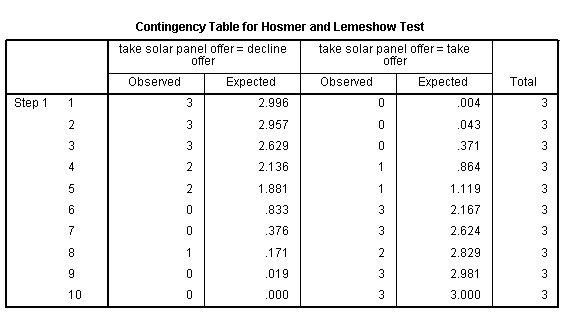
\includegraphics[scale=0.6]{images/Logistic6}\\
		\caption{Hosmer and Lemeshow Table}
	\end{center}
\end{figure}
\newpage
\subsection{R Squared Diagnostics}
\begin{itemize}
	\item In order to understand how much variation in the dependent variable can be explained by the model (the equivalent of $R^2$ in multiple regression), you sho$R^2$uld consult Model Summary statistics.
	
	\item The SPSS output table below contains the \textit{Cox \& Snell R Square} and \textit{Nagelkerke R Square }values, which are both methods of calculating the explained variation. These values are sometimes referred to as pseudo $R^2$ values (and will have lower values than in multiple regression).
	\item  However, they are interpreted in the same manner, but with more caution. Therefore, the explained variation in the dependent variable based on our model ranges from 24.0\% to 33.0\%, depending on whether you reference the Cox \& Snell $R^2$ or Nagelkerke $R^2$ methods, respectively. 
	
	\item Nagelkerke $R^2$ is a modification of Cox \& Snell $R^2$, the latter of which cannot achieve a value of 1. For this reason, it is preferable to report the Nagelkerke $R^2$ value.
\end{itemize}

\begin{figure}[h!]
	\centering
	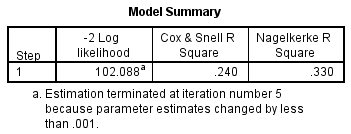
\includegraphics[width=0.9\linewidth]{images/BLogReg-Rsq}
	\caption{SPSS output}
	\label{fig:BLogReg-Rsq}
\end{figure}







\subsection{Pseudo R-squares}
Cox \& Snell R Square and Nagelkerke R Square are two measures from the \textbf{pseudo R-squares} family of measures.

Logistic regression does not have an equivalent to the R-squared that is found in OLS regression; however, many researcehrs have tried to come up with one. 

There are a wide variety of pseudo-R-square statistics (these are only two of them).  Because this statistic does not mean what R-squared means in OLS regression (the proportion of variance explained by the predictors), we suggest interpreting this statistic with great caution.
\subsection{Pseudo-R Squared}
Cox  and Snell R Square and Nagelkerke R Square - These are pseudo R-squares.  Logistic regression does not have an equivalent to the R-squared that is found in OLS regression; however, many people have tried to come up with one.  

\subsubsection{Cox \& Snell R Square}
Cox and Snell's R-Square is an attempt to imitate the interpretation of multiple R-Square based on the likelihood, but its maximum can be (and usually is) less than 1.0, making it difficult to interpret. It is part of SPSS output.

\subsubsection{Nagelkerke's R-Square}
Nagelkerke's R-Square is a further modification of the Cox and Snell coefficient to assure that it can vary from 0 to 1. Nagelkerke's R-Square will normally be higher than the Cox and Snell measure. It is part of SPSS output and is the most-reported of the R-squared estimates.
\newpage



%---------------------------------------------------------- %
\newpage
\subsection{Logistic Regression: Decision Rule}
Our decision rule will take the following form: If the probability of the event is greater than or equal to some threshold, we shall predict that the event will take place. By default, SPSS sets this threshold to .5. While that seems reasonable, in many cases we may want to set it higher or lower than .5.

%---------------------------------------------------------- %

\subsection{SPSS Output}
\begin{itemize}
	\item The variable Vote2005 is a binary variable describing turnout at a general election. The predictor variables are gender and age.
	\begin{center}
		\begin{figure}[h!]
			% Requires \usepackage{graphicx}
			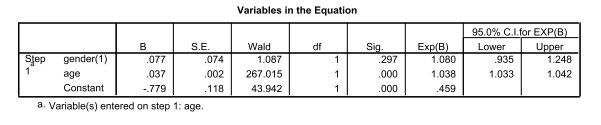
\includegraphics[scale=0.6]{LogWeek10B}\\
			\caption{General Election 2005}
		\end{figure}
	\end{center}
	
	% Image LogWeek10-B
	
	\[\mbox{logit(vote2005)} = -.779 + .077\mbox{gender(1)}+.037\mbox{age}\]
	
	\item The age coefficient is statistically significant. Exp(B) for age is 1.038, which
	means for each year different in age, the person is 1.038 times more likely to turn
	out to vote, having allowed for gender in the model. Eg. a 21 year old is 1.038
	times as likely to turn out to vote than a 20 year old. \item This might not seem much
	of a difference but a 20 year difference leads to a person being $1.038^20 = 2.11$
	times more likely to turn out to vote. E.g. a 40 year old is 2.11 times more likely to
	turn out to vote than a 20 year old, having allowed for gender in the model.
	
	
	\item The gender coefficient is not statistically significant.
	
	
\end{itemize}

%-------------------------------------------%


\subsection{Hosmer-Lemeshow Prostate Example}
We will now consider a real life example to demonstrate Logistic Regression. This example is taken from a Prostate Cancer Study from Hosmer and Lemeshow (2000). The goal of the analysis is to determine if variables
measured at baseline can predict whether a tumour has penetrated the prostatic capsule. The variables are as follows:
\begin{center}
	\begin{figure}[h!]
		% Requires \usepackage{graphicx}
		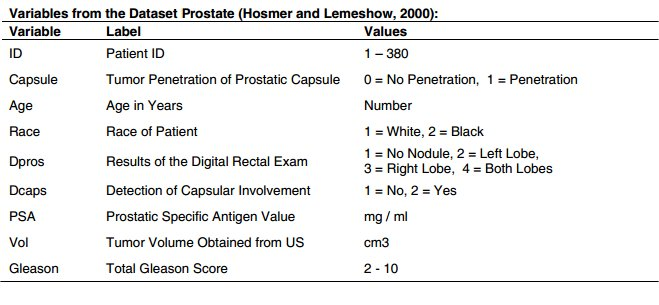
\includegraphics[scale=0.6]{LogWeek10C}\\
		\caption{Variables}
	\end{figure}
\end{center}
\subsection{Kasser and Bruce Infarction Data Example}
We use a set of coronary data (Kasser and Bruce, 1969;
Kronmal and Tarter, 1974) to see if age, history of angina pectoris (ANGINA:
yes, no), history of high blood pressure (HIGHBP: yes, no), and functional class
(FUNCTION: none, minimal, moderate, and more than moderate) can be used to
predict the probability of past myocardial infarction (INFARCT: yes, no).



\subsection{The Likelihood Ratio Test}
The likelihood ratio test to test this hypothesis is based on the likelihood
function. We can formally test to see whether inclusion of an explanatory variable in a model tells us
more about the outcome variable than a model that does not include that variable. Suppose
we have to evaluate two models. 
\begin{center}
	\begin{figure}[h!]
		% Requires \usepackage{graphicx}
		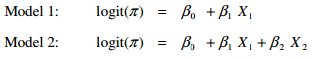
\includegraphics[scale=0.75]{LogWeek10D}\\
		\caption{Variables}
	\end{figure}
\end{center}
Here, Model 1 is said to be nested within Model 2 � all the explanatory variables in Model 1
(X1) are included in Model 2. We are interested in whether the additional explanatory
variable in Model 2 ($X_2$) is required, i.e. does the simpler model (Model 1) fit the data just as
well as the fuller model (Model 2). In other words, we test the null hypothesis that $\beta_2 = 0$
against the alternative hypothesis that $\beta_2 \neq 0$. 

\subsection{Multinomial Logistic Regression}
Multinomial Logistic Regression is useful for situations in which you want to be able to classify
subjects based on values of a set of predictor variables. This type of regression is similar to logistic
regression, but it is more general because the dependent variable is not restricted to two categories.
For Example, In order to market films more effectively, movie studios want to predict what type of
film a moviegoer is likely to see. By performing a Multinomial Logistic Regression, the studio
can determine the strength of influence a person�s age, gender, and dating status has upon the type
of film they prefer. The studio can then slant the advertising campaign of a particular movie
toward a group of people likely to go see it.
%-------------------------------------------------------------------------------------%
\newpage
\section{Binary Classification}	


\subsection{Category Prediction Table}

\begin{itemize}
	\item It is very common to use binomial logistic regression to predict whether cases can be correctly classified (i.e., predicted) from the independent variables. Therefore, it becomes necessary to have a method to assess the effectiveness of the predicted classification against the actual classification.
	\item  There are many methods to assess this with their usefulness oftening depending on the nature of the study conducted. However, all methods revolve around the observed and predicted classifications, which are presented in the ``\texttt{Classification Table}", as shown below:
	
	
	\begin{figure}
		\centering
		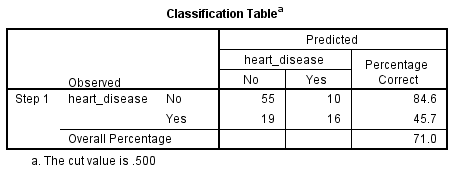
\includegraphics[width=0.8\linewidth]{images/BLogReg-Table}
	\end{figure}
	
	
	
	\item Firstly, notice that the table has a subscript which states, ``\texttt{The cut value is .500}". This means that if the probability of a case being classified into the ``\textbf{\textit{yes}}" category is greater than .500, then that particular case is classified into the ``\textbf{\textit{yes}}" category. 
	Otherwise, the case is classified as in the ``\textbf{\textit{no}}" category. 
\end{itemize}




\subsection{Classification Table}
Rather than using a goodness-of-fit statistic, we often want to look at the proportion of cases we have managed to classify correctly. For this we need to look at the classification table printed out by SPSS, which tells us how many of the cases where the observed values of the dependent variable were 1 or 0 respectively have
been correctly predicted.

In the Classification table, the columns are the two predicted values of the dependent, while the rows are the two observed (actual) values of the dependent. In a perfect model, all cases will be on the diagonal and the
overall percent correct will be 100\%. In this study, 87.5\% were correctly classified for the take offer group and 92.9\% for the decline offer group. Overall 90\% were correctly classified. This is a considerable improvement on the 53.3\% correct classification with the constant model so we know that the model with predictors is a significantly better mode.
\begin{figure}[h!]
	\begin{center}
		% Requires \usepackage{graphicx}
		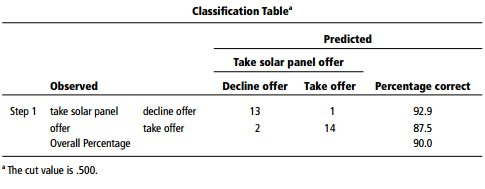
\includegraphics[scale=0.6]{images/Logistic7}\\
		\caption{Classification Table}
	\end{center}
\end{figure}

\subsection{Classification Plot} 
The classification plot or histogram of predicted probabilities
provides a visual demonstration of the correct and incorrect predictions. Also called the `\texttt{classplot}' or the `\texttt{plot of observed groups and predicted probabilities}?,it is another very useful piece of information from the SPSS output when one chooses
\texttt{Classification plots}' under the Options button in the Logistic Regression dialogue box.

\subsection{Interpreting the Classifcation Table}
Whilst the classification table appears to be very simple, it actually provides a lot of important information about your binomial logistic regression result, including:


\begin{itemize}
	\item[A.] The \textbf{percentage accuracy in classification (PAC)}, which reflects the percentage of cases that can be correctly classified as "no" heart disease with the independent variables added (not just the overall model).
	\item[B.] \textbf{Sensitivity}, which is the percentage of cases that had the observed characteristic (e.g., "yes" for heart disease) which were correctly predicted by the model (i.e., true positives).
	\item[C.] \textbf{Specificity}, which is the percentage of cases that did not have the observed characteristic (e.g., "no" for heart disease) and were also correctly predicted as not having the observed characteristic (i.e., true negatives).
	\item[D.] The \textbf{positive predictive value}, which is the percentage of correctly predicted cases "with" the observed characteristic compared to the total number of cases predicted as having the characteristic.
	\item[E.] The \textbf{negative predictive value}, which is the percentage of correctly predicted cases ``without" the observed characteristic compared to the total number of cases predicted as not having the characteristic.
\end{itemize}
%--------------------------------------------------------------------------------------%




\section{Stepwise Logistic Selection}
Stepwise logistic regression involves the stepwise (or one-by-one) selection of variables,
providing a fast and effective method to screen a large number of variables, and to fit
multiple logistic regression equations simultaneously.

In stepwise selection, an attempt is made to remove any insignificant variables from the model before adding a significant variable to the model.

Stepwise binary logistic regression is very similar to stepwise multiple regression in terms of its advantages and disadvantages. Stepwise logistic regression is designed to find the \textbf{\textit{most parsimonious}} set of predictors that are most effective in predicting the dependent variable.

\subsection{Procedure for Stepwise Selection}
Variables are added to the logistic regression equation one at a time, using the statistical criterion of reducing the \textbf{\textit{-2 Log Likelihood error}} for the included variables. (Recall: The lower the -2LL value, the better the fit of the model).

After each variable is entered, each of the included variables are tested to see if the model would be better off the variable were excluded. This does not happen often.

The process of adding more variables stops when all of the available variables have been included or when it is not possible to make a statistically significant reduction in -2 Log Likelihood using any of the variables not yet included.

Categorical variables are added to the logistic regression as a group. It is possible, and often likely, that not all of the individual dummy-coded variables will have a statistically significant individual relationship with the dependent variable. 
%We limit our interpretation to the dummy-coded variables that do have a statistically significant individual relationship.
\subsection{SPSS Implementation}
SPSS provides a table of variables included in the analysis and a table of variables excluded from the analysis.  It is possible that none of the variables will be included.  It is possible that all of the variables will be included.

The order of entry of the variables can be used as a measure of relative importance.

Once a variable is included, its interpretation in stepwise logistic regression is the same as it would be using other methods for including variables.
%-------------------------------------------------------%
\subsection{Advantages and Disadvantages}
\begin{itemize}
	\item Stepwise logistic regression can be used when the goal is to produce a predictive model that is parsimonious and accurate because it excludes variables that do not contribute to explaining differences in the dependent variable.
	
	\item Stepwise logistic regression is less useful for testing hypotheses about statistical relationships. Its usage is recommended only for exploratory purposes, rather that as a formal procedure.
	
	\item Stepwise logistic regression can be useful in finding relationships that have not been tested before. Its findings invite one to speculate on why an unusual relationship makes sense.
	
	\item It is not legitimate to do a stepwise logistic regression and present the results as though one were testing a hypothesis that included the variables found to be significant in the stepwise logistic regression.
	
	\item Using statistical criteria to determine relationships is vulnerable to over-fitting the data set used to develop the model at the expense of generalisability.
	
\end{itemize}
%========================================================%
\begin{quote}
	Menard (1995: 54) writes, "there appears to be general agreement that the use of computer-controlled stepwise procedures to select variables is inappropriate for theory testing because it capitalizes on random variations in the data and produces results that tend to be idosyncratic and difficult to replicate in any sample other than the sample in which they were originally obtained."
\end{quote}
%-------------------------------------------------------%
\subsection{Forward Selection}
You can estimate models using block entry of variables or any of the following stepwise
methods: forward conditional, forward LR, forward Wald, backward conditional, backward
LR, or backward Wald.


Forward selection is the usual option for a stepwise regression,
starting with the constant-only model and adding variables one at a time. The forward
stepwise logistic regression method utilizes the likelihood ratio test which tests the change in �2LL between steps to determine automatically which variables to add or drop from the model.

Method selection allows you to specify how independent variables are entered into the analysis.
Using different methods, you can construct a variety of regression models from the same set of
variables.

\begin{itemize}
	\item[1] Enter. A procedure for variable selection in which all variables in a block are entered in a
	single step.
	\item[2] Forward Selection (Conditional). Stepwise selection method with entry testing based on
	the significance of the score statistic, and removal testing based on the probability of a
	likelihood-ratio statistic based on conditional parameter estimates.
	\item[3] Forward Selection (Likelihood Ratio). Stepwise selection method with entry testing based
	on the significance of the score statistic, and removal testing based on the probability of a
	likelihood-ratio statistic based on the maximum partial likelihood estimates.  (LR stands for Likelihood Ratio and  is considered the criterion least prone to error.)
	\item[4] Forward Selection (Wald). Stepwise selection method with entry testing based on the
	significance of the score statistic, and removal testing based on the probability of the Wald
	statistic.
	\item[5] Backward Elimination (Conditional). Backward stepwise selection. Removal testing is based on
	the probability of the likelihood-ratio statistic based on conditional parameter estimates.
	\item[6] Backward Elimination (Likelihood Ratio). Backward stepwise selection. Removal testing
	is based on the probability of the likelihood-ratio statistic based on the maximum partial
	likelihood estimates.
	\item[7] Backward Elimination (Wald). Backward stepwise selection. Removal testing is based on the
	probability of the Wald statistic.
\end{itemize}
%-------------------------------------------------------%
\subsection{Cross Validation of Stepwise Regression}
When stepwise logistic regression is used, some form of validation analysis is a necessity. We will use 75/25\% cross-validation.

To do cross validation, we randomly split the data set into a 75\% training sample and a 25\% validation sample. We will use the training sample to develop the model, and we test its effectiveness on the validation sample to test the applicability of the model to cases not used to develop it.

In order to be successful, the follow two questions must be answers affirmatively:
Did the stepwise logistic regression of the training sample produce the same subset of predictors produced by the regression model of the full data set?

If yes, compare the classification accuracy rate for the 25\% validation sample to the classification accuracy rate for the 75\% training sample. If the \textbf{shrinkage} (accuracy for the 75\% training sample - accuracy for the 25\% validation sample) is 2\% (0.02) or less, we conclude that validation was successful.

Note: shrinkage may be a negative value, indicating that the accuracy rate for the validation sample is larger than the accuracy rate for the training sample. Negative shrinkage (increase in accuracy) is evidence of a successful validation analysis.

If the validation is successful, we base our interpretation on the model that included all cases.

%\subsection{Model Selection}
%Model selection is a fundamental task in data analysis,
%widely recognized as central to good inference. In many types of statistical software we have 4 automatic model
%selection techniques: forward selection, backward
%elimination, stepwise selection which combines the
%elements of the previous two, and the best subset
%selection procedure. The first three methods are based
%on the same ideas and we will talk only about stepwise
%selection as more flexible and sophisticated selection
%procedure. This choice is subjective, some researchers
%prefer to work with backward selection.
\newpage
\section{Summary of Logistic Regression}
logistic regression or logit regression is a type of regression analysis used for predicting
the outcome of a categorical dependent variable (a dependent variable that can take on a limited number of values,
whose magnitudes are not meaningful but whose ordering of magnitudes may or may not be meaningful)
based on one or more predictor variables.



\begin{itemize}
	\item[(1.)] Logistic regression is intended for the modeling
	of dichotomous categorical outcomes (e.g., characterized by binary responses: buy vs Don't buy, dead vs. alive, cancer vs. none,�).
	
	
	\item[(2.)] We want to predict the probability of a particular response  (0 to 1 scale).
	
	\item[(3.)] For binary responses, linear regression should not be used for several reasons
	but the most common-sense reason is that linear regression can provide predictions NOT on a 0 to 1 scale.
	but rather a predicted response of some numeric value (e.g 2.4 or -800.3).
	
	\item[(4.)] We need a way to link the probabilistic response variable to the continuous and/or categorical predictors and
	keep things on this 0 to 1 scale.
	
	\item[(5.)] Logistic regression winds up transforming the probabilities to odds and then taking the natural logarithm of these odds, called logits.
	
	
	\item[(6.)] Suppose a response variable is passing a test (by convention, 0=no and 1=yes).
	You have 1 predictor - number of days present in class over the past 30 days.
	Suppose the regression coefficient (often just called beta) in the output is 0.14.
	You would then say that, on average, as class presence increases by 1 day, the natural logarithm of the
	odds of passing the test increases by 0.14.
	
	\item[7.)] For the interpretation, you can just talk about the odds.
	Most computer output will give you this number.
	Suppose the answer in odds is 1.24. Then, you just say that,on average, as class presence increases by 1 day,
	the odds of passing the test are multiplied by 1.24.
	In other words, for each additional day present, the odds of passing are 24% greater than that of not passing.
	
	\item[8.)] To validate our findings, normally, we test whether the regression coefficient is equal to zero in the population.
	In logistic regression, the corresponding value for the odds is one (not zero). We got an odds of 1.24.
	Can we trust this? Or should we go with one (which would mean that the odds are the same for both passing and not passing,
	and hence class presence makes no difference at all)?  Look at the p-value (significance). If it less than .05 (by convention), you have enough evidence to reject
	the notion that the odds are really one. You go ahead and support the 1.24 result.
\end{itemize}


%-------------------------------------------%





%---------------------------------------------------------- %
\subsection{Variables in the Equation}
The Variables in the Equation table has several important elements. The Wald statistic and associated probabilities provide an index of the significance of each predictor in the equation.
The simplest way to assess Wald is to take the significance values and if less
than 0.05 reject the null hypothesis as the variable does make a significant contribution.
In this case, we note that family size contributed significantly to the prediction
(p = .013) but mortgage did not (p = .075). The researcher may well want to drop
independents from the model when their effect is not significant by the Wald statistic
(in this case mortgage).

\begin{figure}
\begin{center}
  % Requires \usepackage{graphicx}
  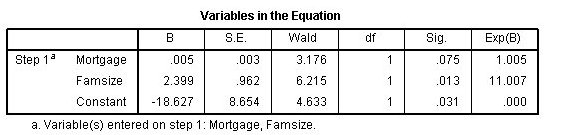
\includegraphics[scale=0.6]{images/Logistic8}\\
  \caption{Variables in the Equation}
\end{center}
\end{figure}

The \textbf{\textit{Exp(B)}} column in the table presents the extent to which raising the corresponding measure by one unit influences the odds ratio. We can interpret \textbf{\textit{Exp(B)}}) in
terms of the change in odds. If the value exceeds 1 then the odds of an outcome occurring increase; if the figure is less than 1, any increase in the predictor leads to a drop in
the odds of the outcome occurring. For example, the \textbf{\textit{Exp(B)}} value associated with
family size is 11.007. Hence when family size is raised by one unit (one person) the
odds ratio is 11 times as large and therefore householders are 11 more times likely to
belong to the take offer group.

The \textbf{\textit{B}} values are the logistic coefficients that can be used to create a predictive
equation (similar to the b values in linear regression) formula seen previously.
\begin{figure}
\begin{center}
  % Requires \usepackage{graphicx}
  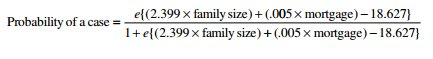
\includegraphics[scale=0.75]{images/Logistic11}\\
  \caption{Logistic Regression Equation}
\end{center}
\end{figure}

Here is an example of the use of the predictive equation for a new case. Imagine a
householder whose household size including themselves was seven and paying
a monthly mortgage of $2,500$ euros. Would they take up the offer, i.e. belong to category 1?
Substituting in we get:
\begin{figure}
\begin{center}
  % Requires \usepackage{graphicx}
  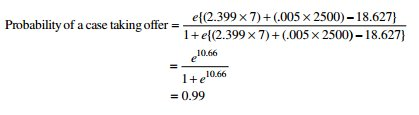
\includegraphics[scale=0.75]{images/Logistic12}\\
  \caption{Logistic Regression Equation : Example}
\end{center}
\end{figure}

Therefore, the probability that a householder with seven in the household and a mortgage of 2,500 p.m. will take up the offer is 99\%, or 99\% of such individuals will be
expected to take up the offer.
Note that, given the non-significance of the mortgage variable, you could be justified
in leaving it out of the equation. As you can imagine, multiplying a mortgage value by
B adds a negligible amount to the prediction as its B value is so small (.005).

\end{document}

\subsection{HSB2 Example}
The hsb2 dataset is taken from a national survey of high school seniors. Two hundred observation were randomly sampled from the High School and Beyond survey. Descriptive statistics and exploratory data analysis are shown below.
Because we do not have a suitable dichotomous variable to use as our dependent variable, we will create one (which we will call honcomp, for honors composition) based on the continuous variable write.  We do not advocate making dichotomous variables out of continuous variables; rather, we do this here only for purposes of this illustration.


Here is the list of variables in the file.
\begin{verbatim}

obs:           200    highschool and beyond (200 cases)
vars:            12    28 Feb 2005 09:25
-----------------------------------------------------------------------------
variable
variable name   type   about the variable
-----------------------------------------------------------------------------
id              scale  student id
female        nominal  (0/1)
race          nominal  ethnicity (1=hispanic 2=asian 3=african-amer 4=white)
ses           ordinal  (1=low 2=middle 3=high)
schtyp        nominal  type of school (1=public 2=private)
prog          nominal  type of program (1=general 2=academic 3=vocational)
read            scale  standardized reading score
write           scale  standardized writing score
math            scale  standardized math score
science         scale  standardized science score
socst           scale  standardized social studies score
hon           nominal  honors english (0/1)
\end{verbatim}
\newpage